\documentclass{oblivoir}
\usepackage{amsmath,amssymb,amsthm,kotex,mdframed,paralist,tabto,pifont}

\counterwithout{subsection}{section}
\newcounter{num}
\newcommand{\prob}[1]
{\bigskip\noindent\refstepcounter{num}\subsection{#1}}

\newcommand{\ans}{
{\par\medskip\begin{mdframed}
\textbf{풀이 : }
\vspace{0.6\textheight}
\end{mdframed}\par
\raggedleft\textbf{답 : (\qquad\qquad\qquad\qquad\qquad\qquad)}
\par}\bigskip\bigskip}

\newcommand\ov[2]{\ensuremath{\overline{#1#2}}}

\newcommand\ve[2]{\ensuremath{\overrightarrow{#1#2}}}

\newcommand{\pa}{\mathbin{\!/\mkern-5mu/\!}}

\TabPositions{0.2\textwidth,0.4\textwidth,0.6\textwidth,0.8\textwidth}
\newcommand\tabb[5]{\par\noindent
\ding{172}{#1}
\tab\ding{173}{#2}
\tab\ding{174}{#3}
\tab\ding{175}{#4}
\tab\ding{176}{#5}}

\newcounter{pnum}
\newcommand\pn{\stepcounter{pnum}\textbf{\thepnum}}

%%%
\begin{document}
\title{혜령 07 - 기하와 벡터[수능특강]\\
{\large 6단원 : 공간도형}}
\author{}
\date{\today}
\maketitle
\tableofcontents

\newpage
%
\prob{06-예제1-1}
그림은 정육면체의 전개도이다.
이 전개도로 만든 정육면체ABED-HOJI에 대해 옳은 것만을 모두 고른 것은?
\begin{enumerate}\tightlist
\item[ㄱ.]
직선 \(AB\)와 직선 \(KM\)는 평행하다.
\item[ㄴ.]
직선 \(AB\)와 직선 \(GN\)은 꼬인 위치에 있다.
\item[ㄷ.]
직선 \(AB\)와 평면 \(DENL\)는 평행하다.
\end{enumerate}
\begin{figure}[h!]
\centering
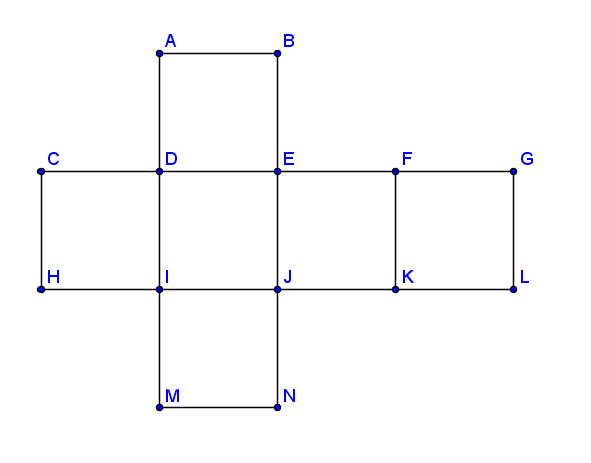
\includegraphics[width=0.7\textwidth]{01}
\end{figure}
\tabb{ㄱ}{ㄴ}{ㄱ,ㄷ}{ㄴ,ㄷ}{ㄱ,ㄴ,ㄷ}
\newpage

%
\prob{06-예제1-2}
그림은 정팔면체의 전개도이다.
이 전개도로 만든 정육면체 CABFGH에 대해 옳은 것만을 모두 고른 것은?
\begin{enumerate}\tightlist
\item[ㄱ.]
직선 \(AB\)와 직선 \(CG\)는 평행하다.
\item[ㄴ.]
직선 \(AB\)와 직선 \(HI\)은 꼬인 위치에 있다.
\item[ㄷ.]
직선 \(AB\)와 평면 \(HIJ\)는 평행하다.
\end{enumerate}
\begin{figure}[h!]
\centering
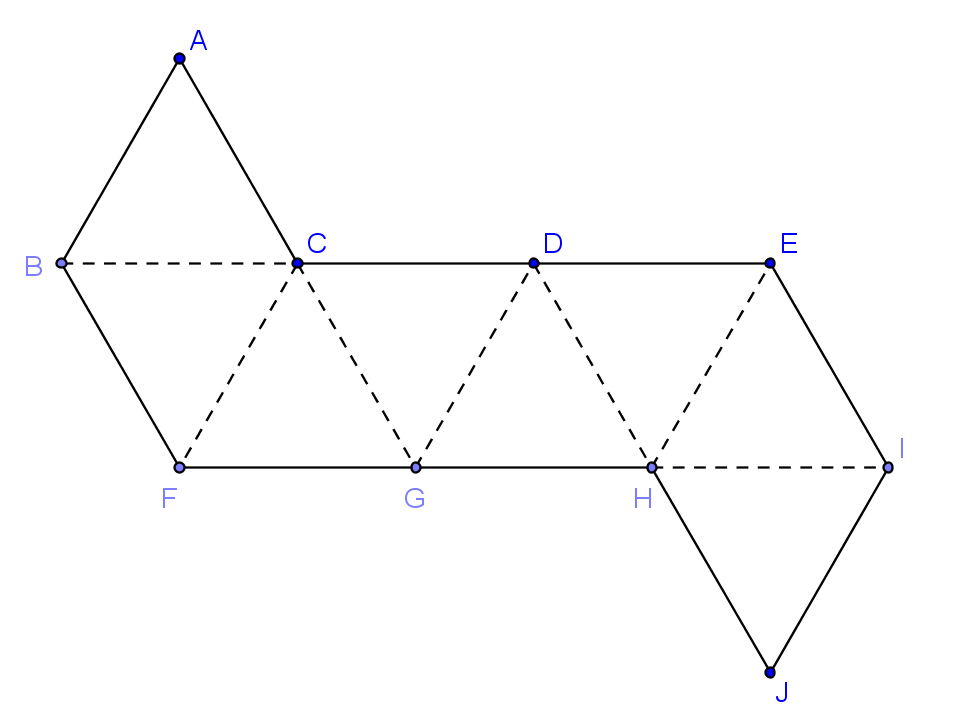
\includegraphics[width=0.7\textwidth]{02}
\end{figure}
\tabb{ㄱ}{ㄴ}{ㄱ,ㄷ}{ㄴ,ㄷ}{ㄱ,ㄴ,ㄷ}
\newpage

%
\prob{06-유제1}
그림과 같은 삼각기둥 ABC-DEF의 각 모서리를 연장한 직선 중 직선 \(AD\)와 평행한 직선의 개수를 \(a\), 직선 \(AD\)와 꼬인 위치에 있는 직선의 개수를 \(b\)라고 할 때, \(a+b\)의 값은?
\begin{figure}[h!]
\centering
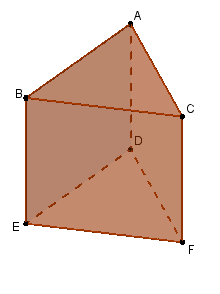
\includegraphics[width=0.35\textwidth]{02a}
\end{figure}
\tabb34567
\newpage

%
\prob{06-예제2}
그림과 같이 정육면체 ABCD-EFGH에서 모서리 \(AB\)의 중점을 \(M\)이라고 하자.
직선 \(AC\)와 직선 \(CF\)이 이루는 예각의 크기를 \(\alpha\), 직선 \(FM\)와 직선 \(CF\)가 이루는 예각의 크기를 \(\beta\),라고 할 때, \(\cos^2\alpha+\cos^2\beta\)의 값을 구하여라.
\begin{figure}[h!]
\centering
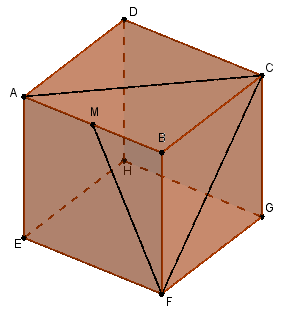
\includegraphics[width=0.4\textwidth]{03a}
\end{figure}
\tabb{\(\frac9{20}\)}{\(\frac12\)}{\(\frac{11}{20}\)}{\(\frac35\)}{\(\frac{13}{20}\)}
\newpage

%
\prob{06-유제3}
그림과 같이 한 모서리의 길이가 2인 정육면체 ABCD-EFGH에서 선분 \(BF\)의 중점을 \(M\)이라고 하자.
직선 \(DE\)와 직선 \(HM\)이 이루는 예각의 크기를 \(\theta\)라고 할 때, \(\cos^2\theta=\frac qp\)이다.
\(p+q\)의 값을 구하시오.
(단, \(p\)와 \(q\)는 서로소인 자연수이다.)
\begin{figure}[h!]
\centering
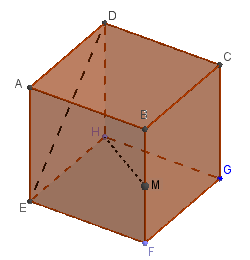
\includegraphics[width=0.4\textwidth]{03}
\end{figure}
\tabb{15}{16}{17}{18}{19}
\newpage

%
\prob{06-유제4}
그림과 같이 밑면인 원의 반지름의 길이가 1이고 높이가 3인 원기둥이 있다. 원기둥의 위쪽에 있는 밑면인 원의 둘레 위의 점 \(P\)와 아래쪽에 있는 밑면인 원의 중심 \(O\)에 대하여 직선 \(PO\)와 수직인 아래쪽에 있는 밑면의 지름을 선분 \(AB\)라고 하자.
평면 \(PAB\)와 원기둥의 밑면이 이루는 예각의 크기를 \(\theta\)라고 할 때, \(\cos\theta\)의 값은?
\begin{figure}[h!]
\centering
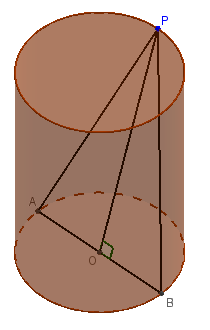
\includegraphics[width=0.37\textwidth]{04}
\end{figure}
\tabb{\(\frac{\sqrt{10}}{10}\)}{\(\frac{\sqrt5}5\)}{\(\frac{\sqrt{30}}{10}\)}{\(\frac{\sqrt3}3\)}{\(\frac{\sqrt2}2\)}
\newpage

%%
%\prob{06-예제5-1}
%그림과 같은 정사면체 ABCD에서 평면 \(ABC\)와 평면 \(BCD\)가 이루는 예각의 크기를 \(\theta\)라고 할 때, \(\cos\theta\)의 값은?
%\begin{figure}[h!]
%\centering
%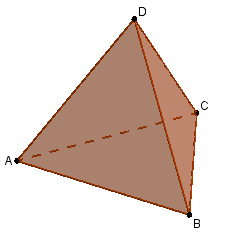
\includegraphics[width=0.4\textwidth]{05a}
%\end{figure}
%\tabb{\(\frac{\sqrt{10}}{10}\)}{\(\frac{\sqrt5}5\)}{\(\frac13\)}{\(\frac{\sqrt3}3\)}{\(\frac{\sqrt2}2\)}
%\newpage
%
%%
%\prob{06-예제5-2}
%그림과 같은 정육면체 ABCD-EFGH에서 선분 \(CG\)의 중점을 \(I\), 선분 \(EF\)의 중점을 \(J\), 선분 \(AD\)의 중점을 \(K\)라고 하자.
%평면 \(IJK\)와 평면 \(EFGH\)가 이루는 예각의 크기를 \(\theta\)라고 할 때, \(\cos\theta\)의 값은?
%\begin{figure}[h!]
%\centering
%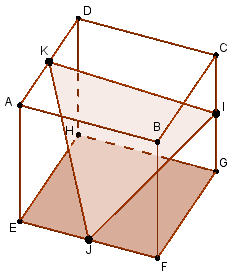
\includegraphics[width=0.4\textwidth]{05}
%\end{figure}
%\tabb{\(\frac{\sqrt{10}}{10}\)}{\(\frac{\sqrt5}5\)}{\(\frac13\)}{\(\frac{\sqrt3}3\)}{\(\frac{\sqrt2}2\)}
%\newpage
%
%%
%\prob{06-기초1}
%그림과 같은 직육면체의 8개의 꼭짓점 중에서 서로 다른 3개의 꼭짓점을 지나는 서로 다른 평면의 개수를 구하시오.
%\begin{figure}[h!]
%\centering
%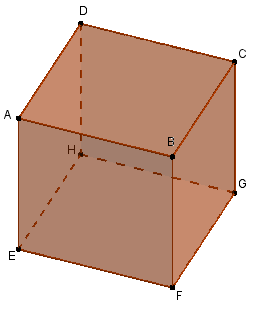
\includegraphics[width=0.4\textwidth]{06}
%\end{figure}
%\tabb{11}{14}{17}{20}{23}
%\newpage

%
\prob{06-기초2-1}
\(\ov AB=\ov AC=3\sqrt5\), \(\ov BC=12\)인 이등변삼각형 ABC에 대해 \(\theta=\angle BAC\)라고 할 때, \(\cos\theta\)의 값을 구하시오.
\begin{figure}[h!]
\centering
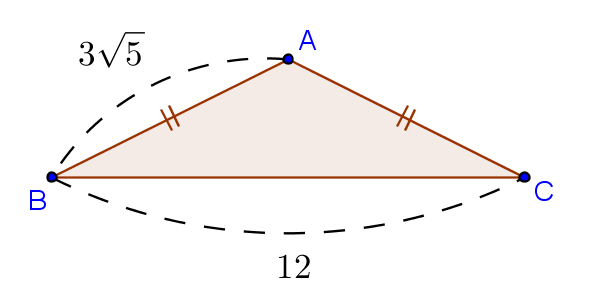
\includegraphics[width=0.4\textwidth]{07}
\end{figure}
\tabb{\(-\frac35\)}{\(-\frac15\)}{\(\frac13\)}{\(\frac15\)}{\(\frac35\)}

%
\prob{06-기초2-2}
\(\ov AB=\ov AC=3\sqrt{10}\)인 이등변삼각형 ABC에 대해 \(A\)에서 선분 BC에 내린 수선의 길이가 \(\sqrt{6}\)이다.
\(\theta=\angle BAC\)라고 할 때, \(\cos\theta\)의 값을 구하시오.
\begin{figure}[h!]
\centering
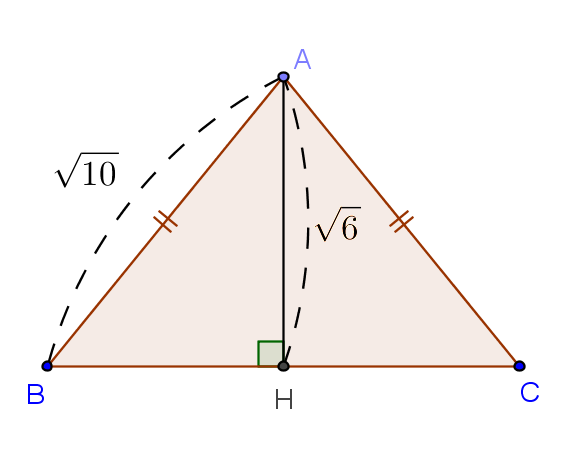
\includegraphics[width=0.4\textwidth]{08}
\end{figure}
\tabb{\(-\frac35\)}{\(-\frac15\)}{\(\frac13\)}{\(\frac15\)}{\(\frac35\)}
\newpage

%
\prob{06-기초2-3}
그림과 같이 모든 모서리의 길이가 \(2\)인 정사면체 \(ABCD\)와 모든 모서리의 길이가 \(2\)인 삼각뿔 \(BCD-EFG\)가 면 \(BCD\)를 공유하고 있다.
선분 \(BC\)의 중점을 \(H\), \(EF\)의 중점을 \(I\)라고 할 때, 직선 \(AH\)와 직선 \(GI\)가 이루는 예각의 크기를 \(\theta\)라고 할 때, \(\cos\theta\)의 값은?
\begin{figure}[h!]
\centering
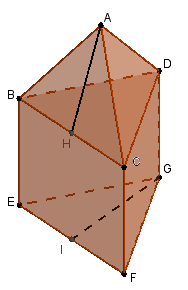
\includegraphics[width=0.4\textwidth]{09}
\end{figure}
\tabb{\(-\frac35\)}{\(-\frac15\)}{\(\frac13\)}{\(\frac15\)}{\(\frac35\)}
\newpage

%
\prob{06-기초3-1}
그림과 같이 평면 \(\alpha\) 위의 서로 다른 두 점 \(A\), \(B\)와 평면 \(\alpha\) 밖의 한 점 \(P\), 점 \(P\)에서 평면 \(\alpha\)에 내린 수선의 발 \(H\)가 있다.
\(\ov AB=3\), \(\ov AP=6\), \(\ov PH=4\), \(\ov AB\perp \ov AP\)일 때, 두 점 \(B\), \(H\) 사이의 거리는?
\begin{figure}[h!]
\centering
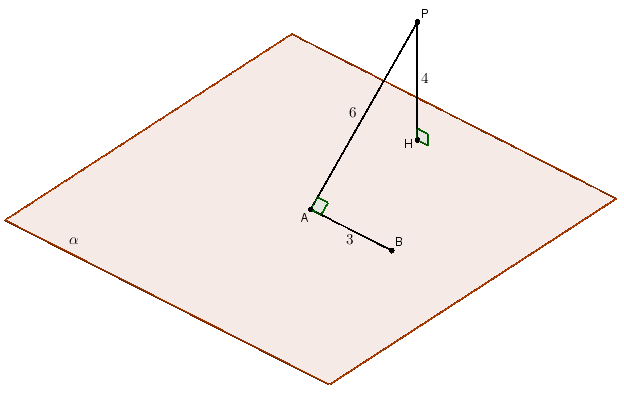
\includegraphics[width=0.9\textwidth]{10}
\end{figure}
\tabb{\(5\)}{\(\sqrt{26}\)}{\(3\sqrt{3}\)}{\(2\sqrt{7}\)}{\(\sqrt{29}\)}
\newpage

%
\prob{06-기초3-2}
그림과 같이 평면 \(\alpha\) 위의 서로 다른 두 점 \(A\), \(B\)와 평면 \(\alpha\) 밖의 한 점 \(P\), 점 \(P\)에서 평면 \(\alpha\)에 내린 수선의 발 \(H\)가 있다.
\(\ov AB=4\), \(\ov AP=5\), \(\ov PH=2\), \(\ov AB\perp \ov AP\)일 때, 두 점 \(B\), \(H\) 사이의 거리는?
\begin{figure}[h!]
\centering
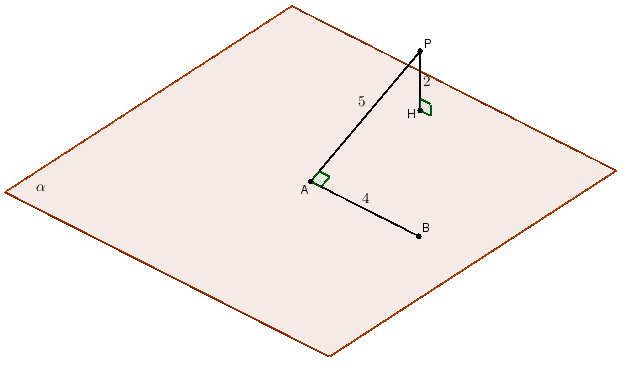
\includegraphics[width=0.9\textwidth]{10a}
\end{figure}
\tabb{\(6\)}{\(\sqrt{37}\)}{\(\sqrt{38}\)}{\(\sqrt{39}\)}{\(2\sqrt{10}\)}
\newpage

%
\prob{06-기초4-1}
그림과 같이 반지름의 길이가 \(5\)인 구의 중심 \(O\)를 지나는 평면 \(\alpha\)와 이루는 각의 크기가 \(30^\circ\)인 평면 \(\beta\)가 있다.
평면 \(\beta\)와 구가 만나서 생기는 단면의 \(\alpha\) 위로의 정사영의 넓이가 \(8\sqrt3\pi\)일 때, 구의 중심 \(O\)와 평면 \(\beta\) 사이의 거리는?
\begin{figure}[h!]
\centering
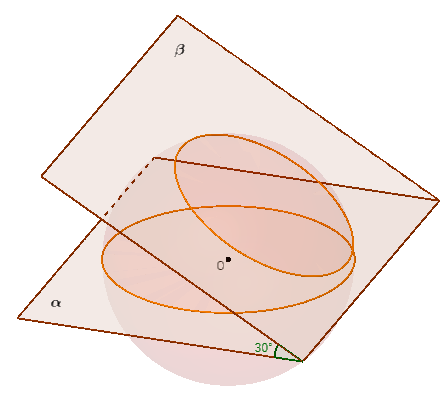
\includegraphics[width=0.7\textwidth]{11}
\end{figure}
\tabb12345
\newpage

%
\prob{06-기본1-1}
서로 다른 세 직선 \(l\), \(m\), \(n\)과 서로 다른 두 평면 \(\alpha\), \(\beta\)에 대하여 옳은 것만을 보기에서 있는 대로 고른 것은?
\begin{enumerate}\tightlist
\item[ㄱ.]
\(l\pa m\)이고 \(m\pa n\)이면 \(l\pa n\)이다.
\item[ㄴ.]
\(l\pa\alpha\)이고 \(l\pa\beta\)이면 \(\alpha\pa\beta\)이다.
\item[ㄷ.]
\(l\pa\alpha\)이고 \(m\pa\alpha\)이면 \(l\pa m\)이다.
\end{enumerate}
\tabb{ㄱ}{ㄴ}{ㄱ,ㄷ}{ㄴ,ㄷ}{ㄱ,ㄴ,ㄷ}

%
\prob{06-기본1-2}
서로 다른 세 직선 \(l\), \(m\)과 서로 다른 두 평면 \(\alpha\), \(\beta\)에 대하여 옳은 것만을 보기에서 있는 대로 고른 것은?
\begin{enumerate}\tightlist
\item[ㄱ.]
\(l\perp\alpha\)이고 \(l\perp\beta\)이면 \(\alpha\pa\beta\)이다.
\item[ㄴ.]
\(l\perp\alpha\)이고 \(m\perp\alpha\)이면 \(l\pa m\)이다.
\item[ㄷ.]
\(l\perp\alpha\)이고 \(m\pa\alpha\)이면 \(l\pa m\)이다.
\end{enumerate}
\tabb{ㄱ}{ㄴ}{ㄱ,ㄴ}{ㄴ,ㄷ}{ㄱ,ㄴ,ㄷ}
\newpage

%
\prob{06-기본2}
그림과 같이 정사면체 \(D-ABC\)와 \(D'-ABC\)가 삼각형 \(ABC\)를 공유한다.
선분 \(AD\)의 중점을 \(M\), 선분 \(AD'\)의 중점을 \(N\), 직선 \(BM\)과 직선 \(BN\)이 이루는 예각의 크기를 \(\theta\)라고 할 때, \(\cos\theta\)의 값은?
\begin{figure}[h!]
\centering
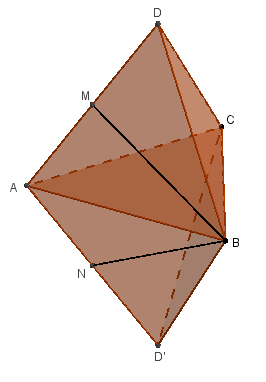
\includegraphics[width=0.45\textwidth]{12}
\end{figure}
\tabb{\(\frac13\)}{\(\frac49\)}{\(\frac59\)}{\(\frac23\)}{\(\frac79\)}
\newpage

%
\prob{06-기본3}
그림과 같이 \(\ov AD=\ov AB=12\)이고 \(\ov AE=6\)인 직육면체 \(ABCD-EFGH\)에서 선분 \(AB\)의 1:2 내분점을 \(I\), 두 선분 \(AC\), \(DI\)의 교점을 \(P\)라고 하자.
직선 \(PE\)와 평면 \(BFGC\)가 이루는 예각의 크기를 \(\alpha\), 두 평면 \(AEP\)와 \(BFGC\)가 이루는 예각의 크기를 \(\beta\)라고 할 때, \(\cos^2\alpha\times\sin^2\beta\)의 값은?
\tabb{\(\frac1{12}\)}{\(\frac16\)}{\(\frac14\)}{\(\frac13\)}{\(\frac5{12}\)}
\begin{figure}[h!]
\centering
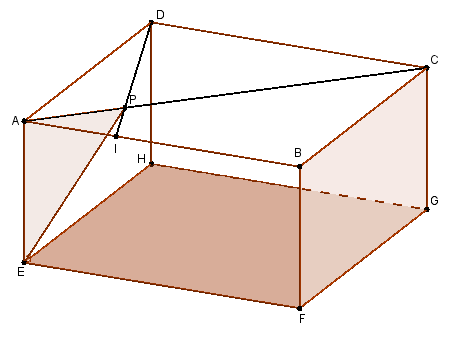
\includegraphics[width=0.8\textwidth]{13}
\end{figure}
\newpage

%
\prob{06-기본4}
그림과 같이 반지름의 길이가 1인 구 \(S_1\)과 반지름의 길이가 2인 두 구 \(S_2\), \(S_3\)이 서로 외접하면서 모두 평면 \(\alpha\)에 접하고 있다.
세 구 \(S_1\), \(S_2\), \(S_3\)의 중심을 각각 \(A\), \(B\), \(C\)라 하고 선분 \(BC\)의 중점을 \(M\)이라고 하자.
직선 \(AM\)과 평면 \(\alpha\)가 이루는 예각의 크기를 \(\theta\)라고 할 때, \(\cos^2\theta=\frac qp\)이다.
\(p+q\)의 값을 구하시오.
(단 \(p\), \(q\)는 서로소인 자연수이다.)
\begin{figure}[h!]
\centering
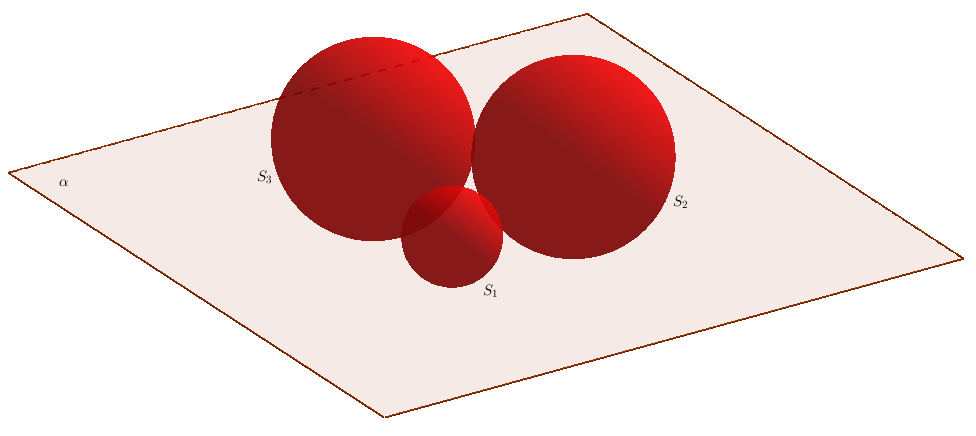
\includegraphics[width=0.99\textwidth]{14}
\end{figure}
\tabb39{15}{21}{27}
\newpage

%
\prob{06-실력1-1}
그림은 \(\ov AB=20\), \(\ov BC=15\)인 직사각형 \(ABCD\)에서 대각선 \(AC\)를 접는 선으로 하여 평면 \(ABC\)와 \(ADC\)가 수직이 되도록 접어서 만든 도형이다.
선분 \(BD\)의 길이를 \(l\)이라고 할 때, \(l^2\)를 구하시오.
\begin{figure}[h!]
\centering
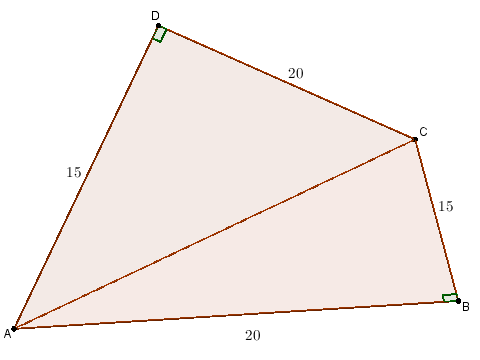
\includegraphics[width=0.8\textwidth]{15}
\end{figure}
\tabb{\(333\)}{\(334\)}{\(335\)}{\(336\)}{\(337\)}
\newpage

%
\prob{06-실력1-2}
그림은 \(\ov AB=8\), \(\ov BC=4\)인 직사각형 \(ABCD\)에서 \(\ov AP=2\)인 선분 \(AB\)위의 점 \(P\), \(\ov CQ=2\)인 선분 \(CD\) 위의 점 \(Q\)에 대하여 선분 \(PQ\)를 접는 선으로 하여 평면 \(APQD\)와 평면 \(BCQP\)가 수직이 되도록 접어서 만든 도형이다.
선분 \(BD\)의 길이는?
\begin{figure}[h!]
\centering
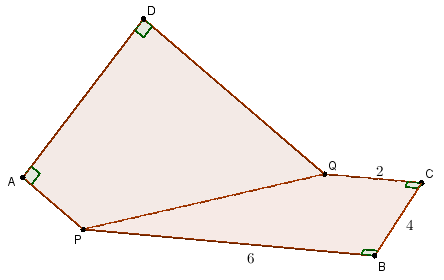
\includegraphics[width=0.8\textwidth]{16}
\end{figure}
\tabb{\(\sqrt{41}\)}{\(\sqrt{42}\)}{\(\sqrt{43}\)}{\(2\sqrt{11}\)}{\(3\sqrt{5}\)}
\newpage

%
\prob{06-실력2}
그림과 같이 \(\ov AC=2\sqrt3\), \(\ov BC=2\sqrt2\), \(\angle BAC=45^\circ\), \(\angle ABC=60^\circ\)인 삼각형 \(ABC\)에 대하여 점 \(A\)를 지나고 직선 \(BC\)와 수직인 직선과 점 \(C\)를 지나고 직선 \(AB\)와 수직한 직선의 교점을 \(H\)라 하고, 점 \(H\)를 지나고 평면 \(ABC\)와 수직인 직선 위의 점을 \(D\)라고 하자. \(\angle ADB=90^\circ\)일 때, 선분 \(DH\)의 길이를 \(d\)라고 하자.
\(d^2\)의 값은?
\begin{figure}[h!]
\centering
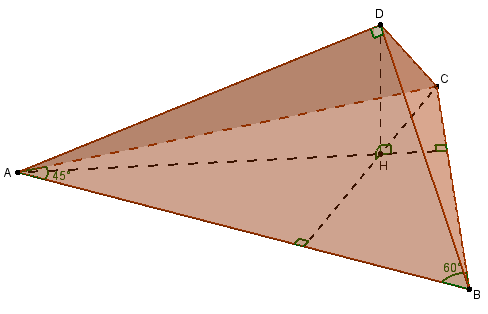
\includegraphics[width=0.8\textwidth]{17}
\end{figure}
\tabb{\(\sqrt3-1\)}{\(\sqrt3\)}{\(\sqrt3+1\)}{\(2\sqrt3-2\)}{\(2\sqrt3+2\)}
\newpage

%%%%
\begin{table}[h!]
\begin{tabular}{|c|c||c|c||c|c||c|c|}
\hline
\pn&\ding{174}	&\pn&\ding{175}	&\pn&\ding{175}	&\pn&\ding{176}\\\hline
\pn&\ding{176}	&\pn&\ding{172}	&\pn&\ding{172}	&\pn&\ding{175}\\\hline
\pn&\ding{174}	&\pn&\ding{176}	&\pn&\ding{173}	&\pn&\ding{174}\\\hline
\pn&\ding{172}	&\pn&\ding{174}	&\pn&\ding{176}	&\pn&\ding{176}\\\hline
\pn&\ding{173}	&\pn&\ding{176}	&\pn&\ding{175}	&\pn&\ding{175}\\\hline
\end{tabular}
\end{table}

\end{document}